
\documentclass[12pt]{article}

% Packages here
\usepackage{geometry}
\usepackage{multicol}
\usepackage{enumitem}
\usepackage{amsmath}
\usepackage{listings}
\usepackage{graphicx}
\usepackage{xcolor}
 
% Configurations here
\definecolor{codegreen}{rgb}{0,0.6,0}
\definecolor{codegray}{rgb}{0.5,0.5,0.5}
\definecolor{codepurple}{rgb}{0.58,0,0.82}
\definecolor{backcolour}{rgb}{0.95,0.95,0.92}
 
\lstdefinestyle{mystyle}{
    backgroundcolor=\color{backcolour},   
    commentstyle=\color{codegreen},
    keywordstyle=\color{magenta},
    numberstyle=\tiny\color{codegray},
    stringstyle=\color{codepurple},
    basicstyle=\ttfamily\footnotesize,
    breakatwhitespace=false,         
    breaklines=true,                 
    captionpos=b,                    
    keepspaces=true,                 
    numbers=left,                    
    numbersep=5pt,                  
    showspaces=false,                
    showstringspaces=false,
    showtabs=false,                  
    tabsize=2
}
 
\lstset{style=mystyle}

\geometry{margin=1cm, bottom=2cm}
\setlength{\columnseprule}{1pt}

% Content here
\begin{document}
  \title{Homework 7}
  \author{Nguyen Tien Duc ITITIU18029}
  \maketitle
  \begin{multicols}{2}
    [\part*{Page 608-609}]
      \section*{6}
        Consider each person at the party a vertice. If that person shakes hands with another person, an edge is created between 2 persons.\\
        The degree of each vertex is the number of people the person represents that vertex shakes hands with.
        By Theorem 1, the sum of the degrees is twice the amount of edges, so the sum of the number of handshakes each person makes is twice the total number of handshakes. \\
        Therefore, the total number of people a person has shaken hands with, over the set of people at the party, is even.
      \section*{10}
        \subsection*{Exercise 7}
          In-degrees = 3 + 1 + 2 + 1 = 7 \\
          Out-degrees = 1 + 2 + 1 + 3 = 7 \\
          And the number of edges is 7
        \subsection*{Exercise 8}
          In-degrees = 2 + 3 + 2 + 1 = 8 \\
          Out-degrees = 2 + 4 + 1 + 1 = 8 \\
          And the number of edges is 8
        \subsection*{Exercise 9}
          In-degrees = 6 + 1 + 2 + 4 + 0 = 13 \\
          Out-degrees = 1 + 5 + 5 + 2 + 0 = 13 \\
          And the number of edges is 13

      \section*{12}
        Degree of a vertex represents the number of acquaintanceship a person has, or the number of people a person knows. \\
        Isolated vertices represents people who knows nobody else. \\
        Pendant vertices represents people who knows only one other person. \\
        If the average degree of a vertex is 1000, then an average person knows 1000 different people.
  \end{multicols}

  \begin{multicols}{2}
    [\part*{Page 618-619}]
    \section*{6}
    \[
    \left[\begin{matrix}
        &a &b &c &d &e \\
      a &0 &1 &0 &1 &0 \\
      b &1 &0 &0 &1 &1 \\
      c &0 &0 &0 &1 &1 \\
      d &1 &1 &1 &0 &0 \\
      e &0 &1 &1 &0 &0
    \end{matrix}\right]
    \]
    \section*{8}
    \[
    \left[\begin{matrix}
        &a &b &c &d &e \\
      a &0 &1 &0 &1 &0 \\
      b &1 &0 &1 &1 &1 \\
      c &0 &1 &1 &0 &0 \\
      d &1 &0 &0 &0 &1 \\
      e &0 &0 &1 &0 &1
    \end{matrix}\right]
    \]
    \section*{14}
    \[
    \left[\begin{matrix}
        &a &b &c &d \\
      a &0 &3 &0 &1 \\
      b &3 &0 &1 &0 \\
      c &0 &1 &0 &3 \\
      d &1 &0 &3 &0
    \end{matrix}\right]
    \]
    \section*{56}
      \begin{center}
        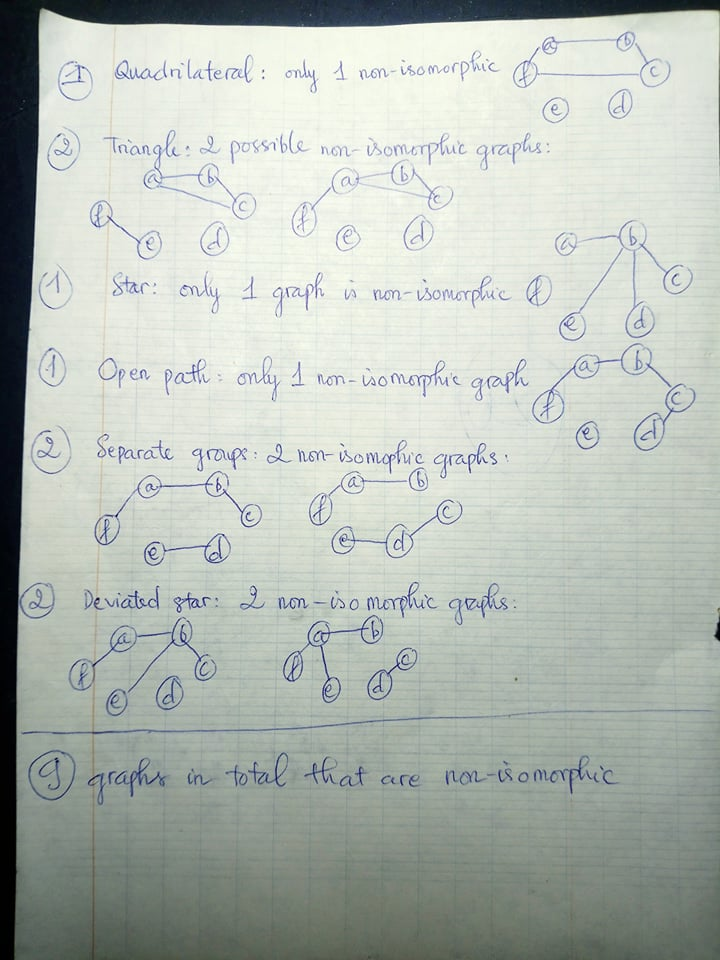
\includegraphics[width=10cm]{56.jpg}
      \end{center}
  \end{multicols}

  \begin{multicols}{2}
    [\part*{Page 644-645}]
    \section*{10}
      We can model this problem using graph theory, the vertices are the lands:
      \begin{itemize}
        \item Vertice N: northern bank
        \item Vertice S: southern bank
        \item Vertice L: left island
        \item Vertice R: right island
      \end{itemize}
      The bridges are the edges between vertices.
      \[
      \left[\begin{matrix}
          &N &S &L &R \\
        N &0 &1 &1 &0 \\
        S &1 &0 &2 &1 \\
        L &1 &2 &0 &1 \\
        R &0 &1 &1 &0
      \end{matrix}\right]
      \]
      As shown in the matrix, each of the piece of land is connected to an even number of other lands.\\
      Therefore, there must be an Euler circuit for this graph.\\
      In conclusion, a person can cross all bridges exactly once and return to the starting point.
    \section*{14}
      \begin{center}
        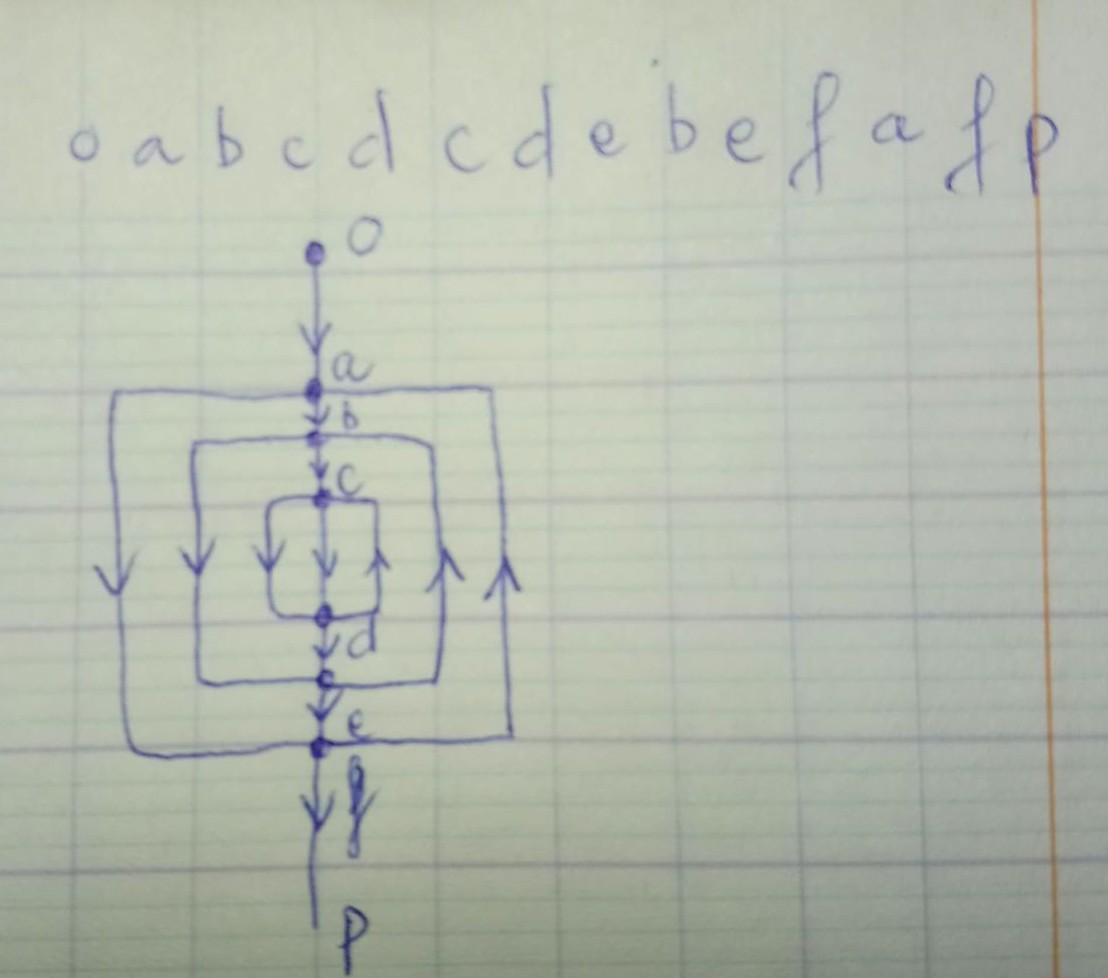
\includegraphics[width=8cm]{14.jpg};
      \end{center}
      We can represent the picture as a graph. As shown the above figure, there are 8 vertices.\\
      All of the vertices have equal number of in-degrees and out-degrees except for only 2 vertices, o and p. \\
      Therefore, there is no Euler circuit for this graph but there is still an Euler path.\\
      Therefore, we can draw this picture in a continuous motion without lifting the pencil.
    \section*{16}
      Suppose the directed multigraph has an Euler circuit. Then, the graph must be strongly connected, thus, also weakly connected.\\
      We can count the in-degrees and out-degrees by following the circuit: as the circuit pass through a vertex, it adds one to the count of both the in-degrees and out-degrees as it comes in and out of every vertex. Therefore, number of in and out degrees of each vertex are equal.\\
      Reversely, if the go against what have been stated, the number of in and out degrees are different, then the circuit can just go in but cannot leave a vertex or cannot even go in a vertex.\\
      Therefore, the statement is proved.
    \section*{22}
      Since vertice b has 4 in-degrees and 3 out-degrees and vertice c has 2 in-degrees, 3 out-degrees, this graph firstly does not satisfy the condition in problem 16.//
      However, all the other vertices have the same number of in-degrees and out-degrees, thus making the graph satisfy the condition in problem 17.//
      Therefore, the graph has an Euler path but not an Euler circuit.//
      As c has more outs than ins while b has more ins than outs, the Euler path must go in the direction from c to b.\\
      One Euler path is: c e b d c b f d e f e a f a b c b
  \end{multicols}

  \part*{Euler Circuit Algorithm}
    \section*{Code:}
      \lstinputlisting[language=c++]{EulerCircuit.cpp}
    \section*{Demo:}
      \begin{center}
        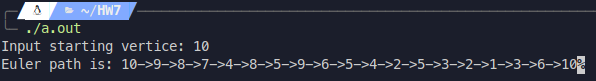
\includegraphics{EulerResult.png};
      \end{center}

\end{document}
